%-------------------------
%minimal-unix
%(c) H.Buchmann FHNW 2014
%export TEXINPUTS=${HOME}/fhnw/edu/:${HOME}/fhnw/edu/tinL/config/latex:${HOME}/fhnw/edu/config//:
%-------------------------
\documentclass{beamer}
\usepackage{latex/beamer}
%---------------------
%local defines
%(c) H.Buchmann FHNW 2009
%$Id$
%---------------------
\newcommand{\target} {\beaglebone\xspace}
\newcommand{\targetS}{{\bf BBG}\xspace}
\newcommand{\host}   {{\em Host}\xspace}
\newcommand{\targetroot} {{\bf target-root}\xspace}
\newcommand{\kernel} {{\bf kernel}\xspace}
\renewcommand{\c}{{\bf C}\xspace}
\newcommand{\cpp}{{\bf C++}\xspace}
\newcommand{\posix}{{\bf POSIX}\xspace}

\input{/home/buchmann/latex/dirtree/dirtree.tex}

\usepackage[absolute]{textpos}
\setlength{\TPHorizModule}{1mm}
\setlength{\TPVertModule}{1mm}

\begin{document}

\newcommand{\qemu}{{\em qemu}\xspace}
\newcommand{\busybox}{{\em busybox}\xspace}
\newcommand{\yocto}{{\em yocto}\xspace}
\title[\yocto]{\yocto\\\linux nach Mass ?}

\frame{\titlepage}
\begin{frame}{Um was geht es ?}
 \begin{itemize}
  \item Massgeschneidertes \linux f�r:
  \begin{itemize}
   \item heterogene Hardwareplatformen
   \item eingebettete Systeme
  \end{itemize}
  \item mit 
  \begin{itemize}
   \item standardisierter (einfacher ?) Herstellung
  \end{itemize}
 \end{itemize}
\end{frame}

\section{The Big Picture}
\begin{frame}{The Big Picture}{\linux \& Co.}
 \begin{block}{einerseits}
  \begin{itemize}
   \item besteht \linux aus nur ein paar Komponenten
   \item ist \linux relativ modern
  \end{itemize}
 \end{block}
 \begin{block}{andrerseits}
  \begin{itemize}
   \item ist \linux sehr komplex
   \item ist \linux klassisch hergestellt
   \begin{itemize}
    \item mit �ber 30-j�hrigen Konzepten
   \end{itemize}
  \end{itemize}
 \end{block}
\end{frame}

\begin{frame}{Die Komponenten}{layers}
\begin{center}
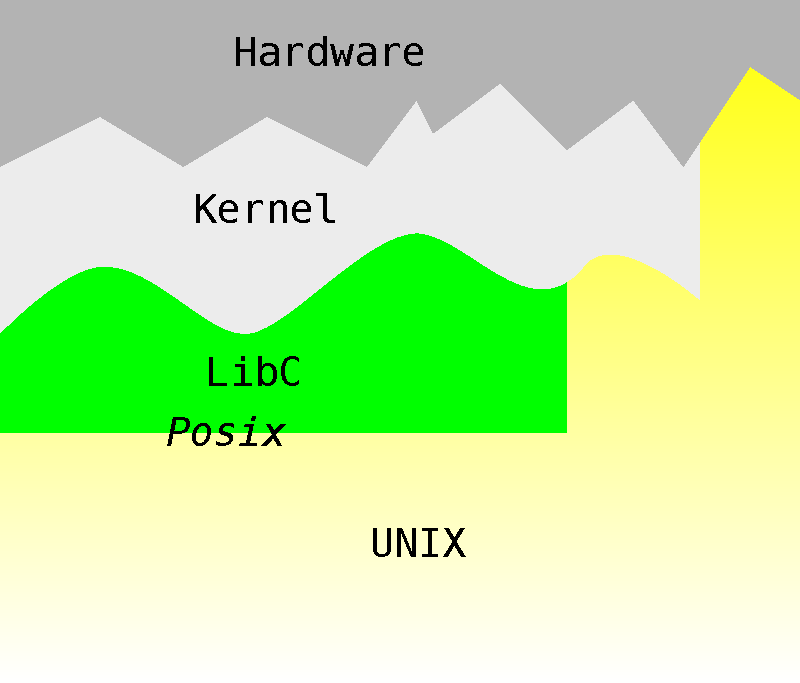
\includegraphics[width=9cm]{layers.pdf}
\end{center}
\end{frame}

\begin{frame}{Die Komponenten}
 \begin{description}
  \item[HW] heterogen:
  \begin{itemize}
   \item Architekturen \arm, {\em Intel}
   \item Peripherie 
  \end{itemize}
  \item[Kernel] das eigentliche \linux
  \begin{itemize}
   \item Sammlung von {\em drivern}
   \item Scheduling
   \item Verwaltung der Resourcen
  \end{itemize}
  \item[LibC] die POSIX Norm
  \begin{itemize}
   \item {\tiny\url{http://pubs.opengroup.org/onlinepubs/9699919799/}}
  \end{itemize}
  \item[\unix] der Rest:
  \begin{itemize}
   \item alles ist ein File
  \end{itemize}
 \end{description}
\end{frame}

\begin{frame}{Die Komplexit�t}
 \begin{block}{Zwei Beispiele}
 \begin{itemize}
   \item die {\em include} Relationen im {\em kernel}
   \item die Verzeichnisstruktur einer \unix Workstation
 \end{itemize}
 \end{block}
\end{frame}

\begin{frame}{Include Relationen}{nur im \kernel}
\vspace{-3.5mm}
\begin{center}
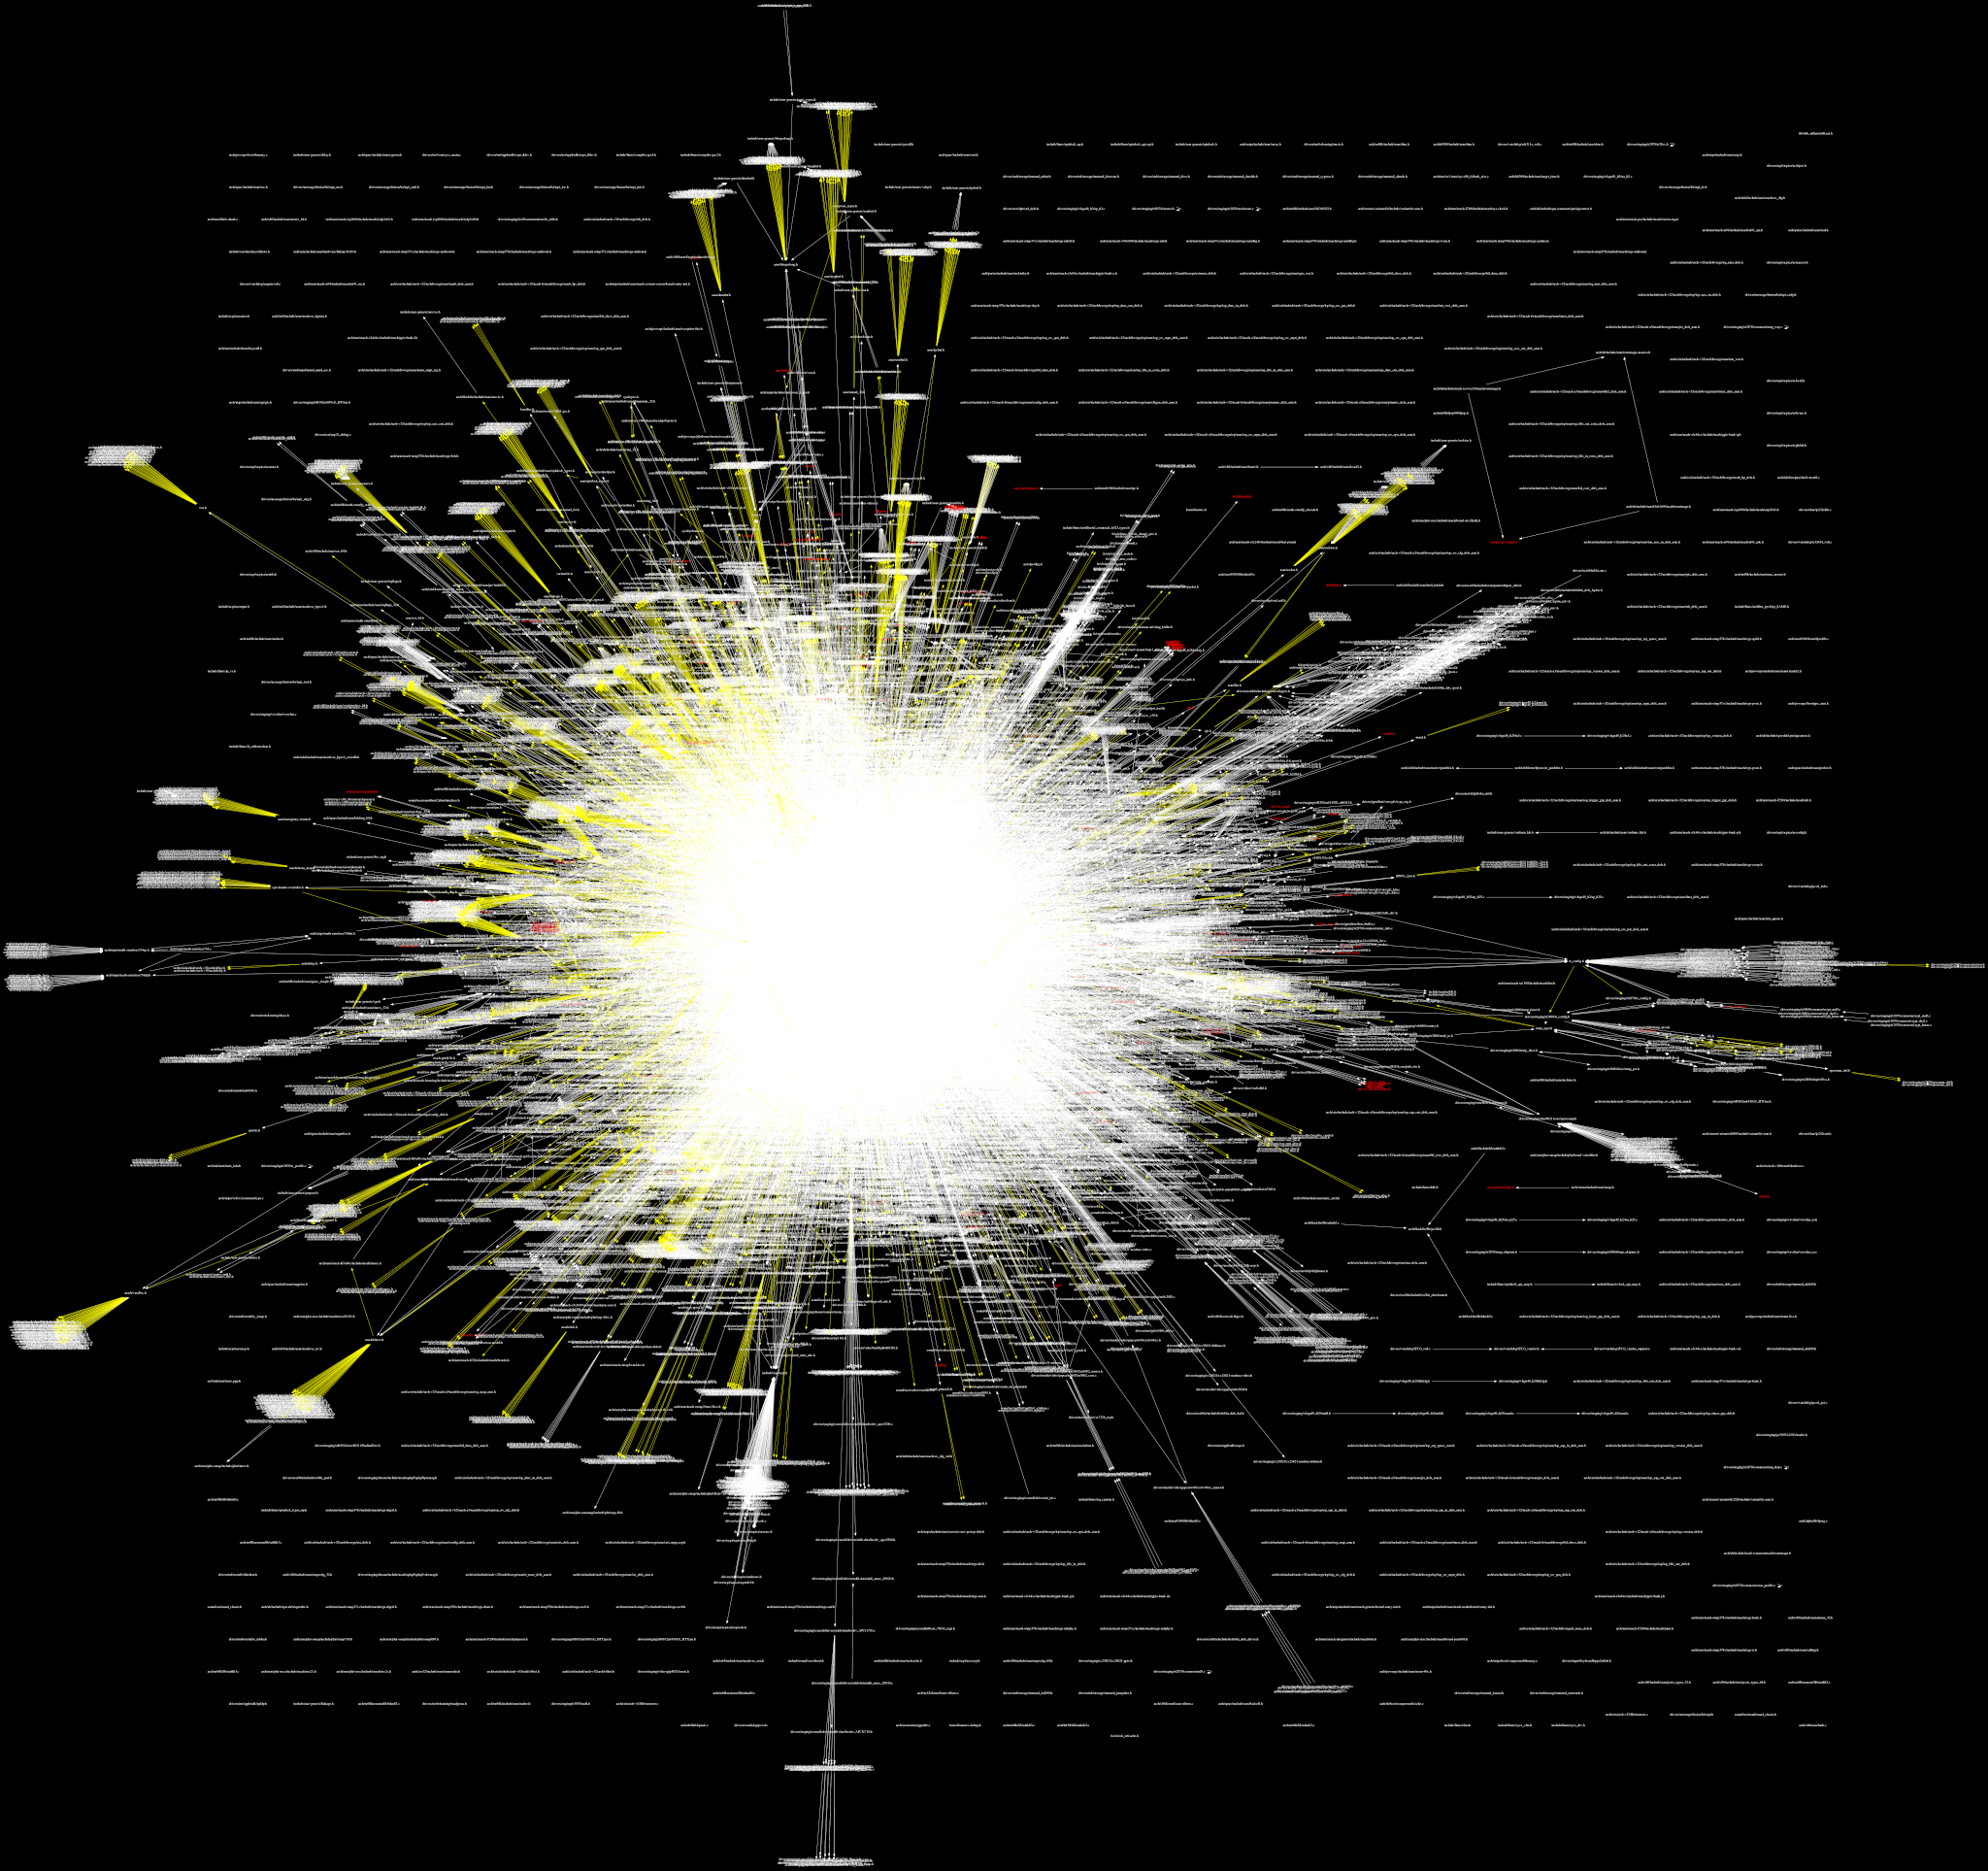
\includegraphics[height=8cm]{include-small.png}
\end{center}
\end{frame}

\begin{frame}{Verzeichnisstruktur}{einer Workstation}
\vspace{-5mm}
\begin{center}
 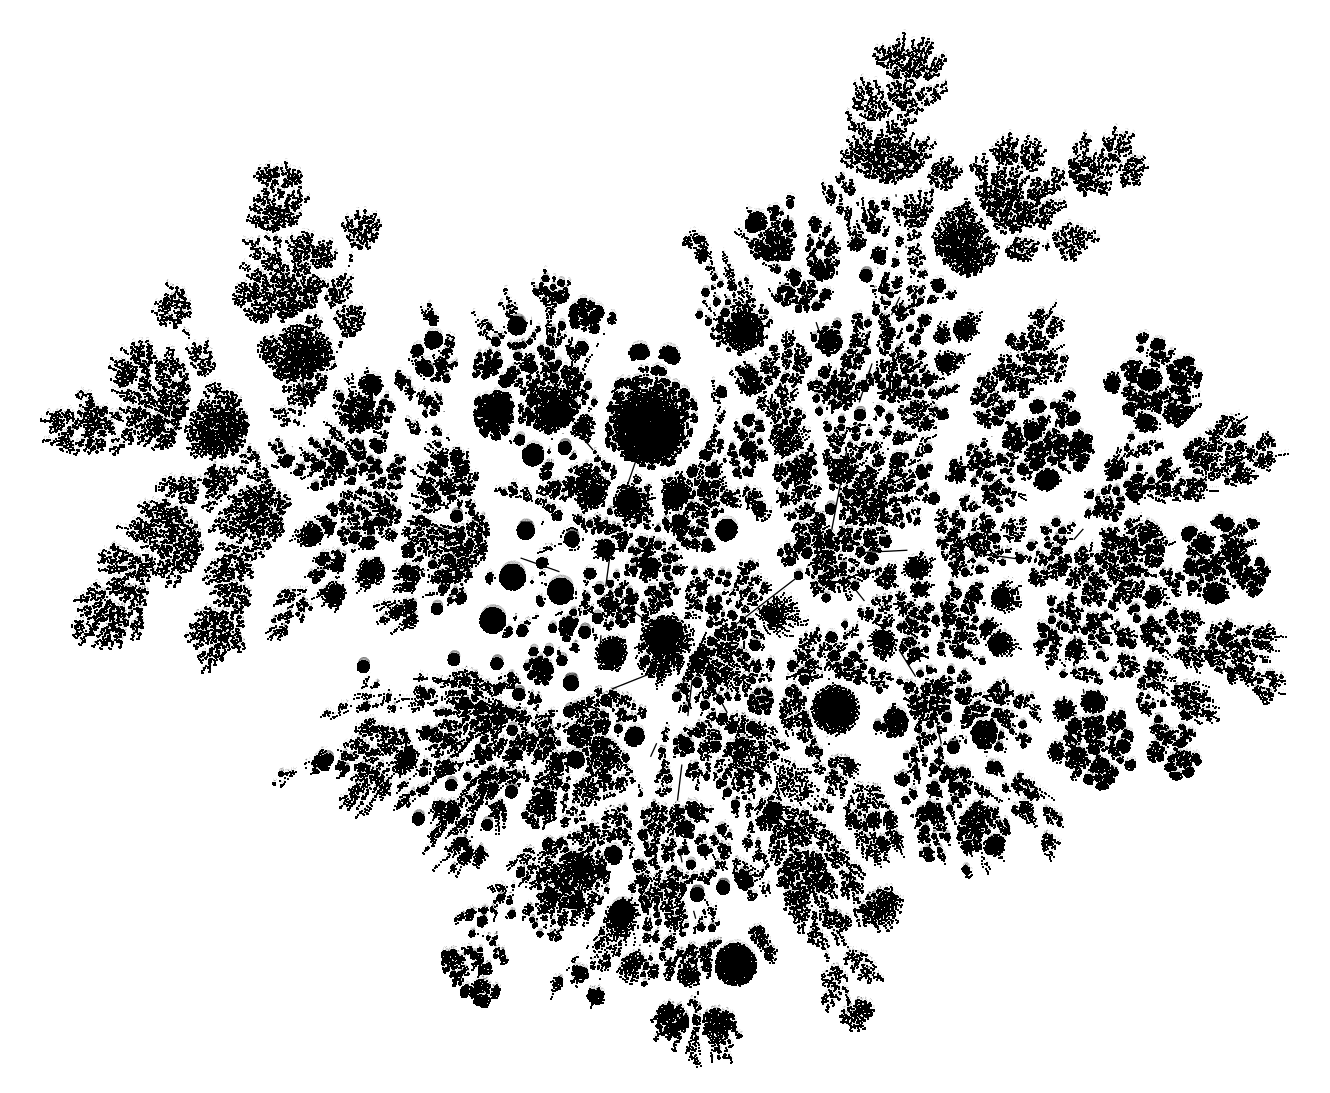
\includegraphics[height=7cm]{directories.png}
\end{center}
\end{frame}

\begin{frame}{Die Herstellung}{die klassischen Methoden}
 \begin{description}[\cod{make}]
  \item[\C] die dominante Programmiersprache
  \item[\cod{make}] Steuerung der Herstellung
 \end{description}
  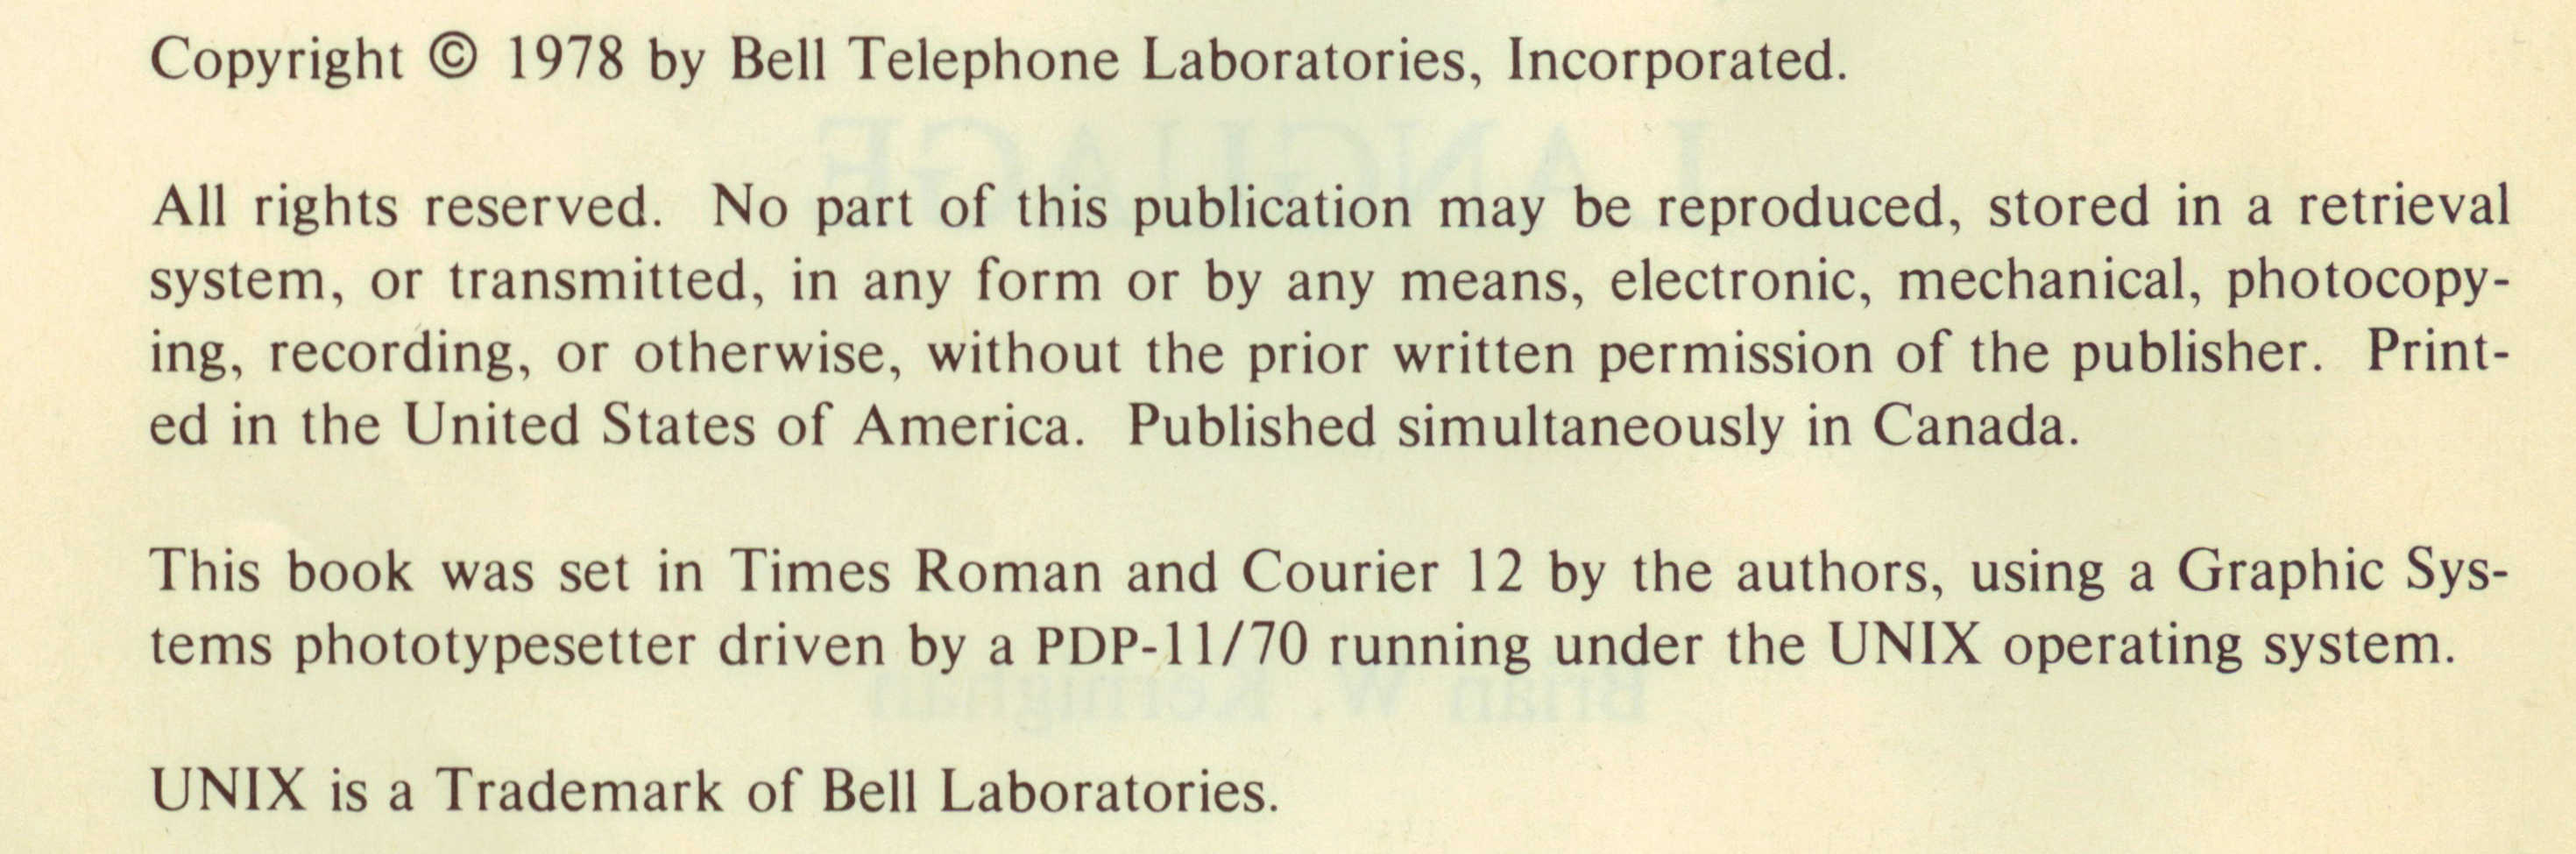
\includegraphics[width=11cm]{copyright.jpg} 
\end{frame}

\begin{frame}{The Big Picture}{Die Herstellung}
 \begin{block}{Gegeben}
  \vspace{-3mm}
  \begin{itemize}
   \item eine Hardware
   \item korrekte\footnote{meistens} Sourcefiles 
   \begin{itemize}
    \item haupts�chlich \C
    \item verstreut auf der Welt
    \item selber geschrieben
   \end{itemize}
  \end{itemize}
 \end{block}
 \vspace{-5mm}
 \begin{block}{Gesucht}
  \vspace{-3mm}
  \begin{itemize}
   \item ein Produkt
   \begin{itemize}
    \item z.B. ein \linux basiertes eingebettetes System
   \end{itemize}
  \end{itemize}
 \end{block}
 \vspace{-5mm}
 \begin{block}{L�sungsweg}
  \vspace{-3mm}
  \begin{itemize}
   \item z.B. \yocto
   \item oder etwas anderes
  \end{itemize}
 \end{block}
\end{frame}

\begin{frame}{Das Problem}{die richtige Wahl}
 \begin{itemize}
  \item die {\Huge richtigen} Sourcefiles
  \item {\Huge richtig} konfiguriert
 \end{itemize}
\end{frame}

\section{\yocto}
\begin{frame}{\yocto}{\url{https://www.yoctoproject.org}}
 \begin{block}{Gegeben}
  \vspace{-3mm}
  \begin{itemize}
   \item eine Hardware
   \item korrekte\footnote{meistens} Sourcefiles 
   \begin{itemize}
    \item haupts�chlich \C
    \item verstreut auf der Welt
    \item selber geschrieben
   \end{itemize}
  \end{itemize}
 \end{block}
 \vspace{-5mm}
 \begin{block}{Gesucht}
  \vspace{-3mm}
  \begin{itemize}
   \item ein Produkt
   \begin{itemize}
    \item z.B. ein \linux basiertes eingebettetes System
   \end{itemize}
  \end{itemize}
 \end{block}
 \vspace{-5mm}
 \begin{block}{L�sungsweg}
  \vspace{-3mm}
  \begin{itemize}
    \item \cod{bitbake {\em theProduct}}
  \end{itemize}
 \end{block}
\end{frame}

\begin{frame}{Wichtige Begriffe}
 \begin{itemize}
  \item Package
  \begin{itemize}
   \item Abh�ngigkeiten
  \end{itemize}
  \item Konfiguration
  \begin{itemize}
   \item die richtige Wahl
  \end{itemize}
  \item Versionen
  \begin{itemize}
   \item z.B. (und vor allem) \cod{git}
  \end{itemize}
  \item{Image}
  \begin{itemize}
   \item das Endprodukt
  \end{itemize}
 \end{itemize}
\end{frame}

\begin{frame}{Wichtige Begriffe}
 \begin{itemize}
  \item Layer
  \begin{itemize}
   \item die Verzeichnisse \cod{meta-*}
  \end{itemize}
  \item SDK Software Development Kit
  \begin{itemize}
   \item die {\em toolchain}
  \end{itemize}
  \item \cod{bitbake}
  \begin{itemize}
   \item das Arbeitspferd
  \end{itemize}
  \item Rezept {\em recipe}
  \begin{itemize}
   \item beschreibt die Herstellung einer Komponente
  \end{itemize}
 \end{itemize}
\end{frame}

\subsection{Demo}
\begin{frame}{Vorbereitung}
{\footnotesize\url{www.yoctoproject.org/docs/1.7/yocto-project-qs/yocto-project-qs.html}}
\begin{itemize}
 \item Installation
 \begin{itemize}
   \item \see{}Getting the Yocto Project
 \end{itemize}
 \item Setze korrekte Umgebung 
  \begin{itemize}
    \item \cod{. oe-init-build-env} 
  \end{itemize}
  \item  Starte
   \begin{itemize}
     \item \cod{bitbake -k core-image-minimal}
     \item braucht Zeit
     \item braucht $\approx 40 GiB$ Festplatte
   \end{itemize}
\end{itemize} 
\end{frame}

\begin{frame}{Das Resultat}{als virtuelle Machine}
\begin{block}{Die Files:}
 \begin{block}{\kernel}
  \cod{bzImage-qemux86.bin}
 \end{block}
 \begin{block}{\unix}
  \cod{core-image-minimal-dev-qemux86-20141018183055.rootfs.ext3}
 \end{block}
\end{block}
\begin{block}{Starten}
 \cod{runqemu qemux86 {\em kernel} {\em unix}  serial}
\end{block}
\remark{predefined:\\ 
{\tiny\url{http://downloads.yoctoproject.org/releases/yocto/yocto-1.7/machines/qemu/qemux86/}}}
\end{frame}

\section{Aufgaben}

\begin{frame}{Ziel}
 \begin{itemize}
  \item \cod{hello-world} auf dem \host und auf dem \targetS
  \item \cod{primes} auf dem \host und auf dem \targetS
 \end{itemize}
\end{frame}


\begin{frame}{The big Picture}
 \begin{itemize}
  \item Source File: \cod{hello-world.cc}
  \item falls es nicht klapt ?
  \begin{itemize}
   \item wo ist der File ?
  \end{itemize}
 \end{itemize}
\end{frame}


%\subsection{Die Programme}
%\begin{frame}{Development}{\cod{hello-world-c.c}}
%\hspace*{-8mm}
%{
%\begin{tabular}{llllll}
% Host & Target & OS & Toolchain & Verbindung & Bemerkungen\\
% \hline
% \targetS & \targetS & Debian & mitgeliefert&&\\
% \host   & \targetS & Debian & \cod{\tiny tc-tinl-gcc-8.1.0-2018.05.21.tar.gz} & sshfs\\
% \host   & \targetS & minimal & \cod{\tiny tc-tinl-gcc-8.1.0-2018.05.21.tar.gz} & SD-Card  &später\\
% \host   & \targetS & minimal & \cod{\tiny tc-tinl-gcc-8.1.0-2018.05.21.tar.gz} & curlftpfs&später\\
%\end{tabular}
%}
%\remark{Toolchain auf der Cloud: \href{https://drive.switch.ch/index.php/s/A6H382zEGDrgfAL}
%       {\Huge tinL}}
%\end{frame}

%layers
\end{document}
